\chapter{Intro}\label{ch:intro}

The boundary between Natural Language Processing (NLP) and Text Generation (TG), or the latest \textit{Neural Text Generation (NTP)}, is relatively blurred and overlap in many ways. Generally speaking, all of the NTG tasks are NLP based, but not all NLP tasks are NTG based.

\section{Difference of NLP and NTG}
In recent months and years, neural networks have produced many \textit{state-of-the-art} results in almost all possible disciplines of machine learning \cite{NTG2}. The roots of Neural Networks (NN) lie down almost 80 years ago in 1943, when \textbf{McCulloch-Pitts} \cite{NN} compared for the first time neuronal networks with the structure of the human brain. This first attempt to approach artificial neurons with neurons from the brain lead to the nowadays commonly used understanding of a simple neuron of a basic neural network (shown in figure \ref{neuron}). Those neurons connected together create an aritificial neuronal network, which can calculate any possible logical or arithmetic function. 

\begin{figure}
  \begin{center}
  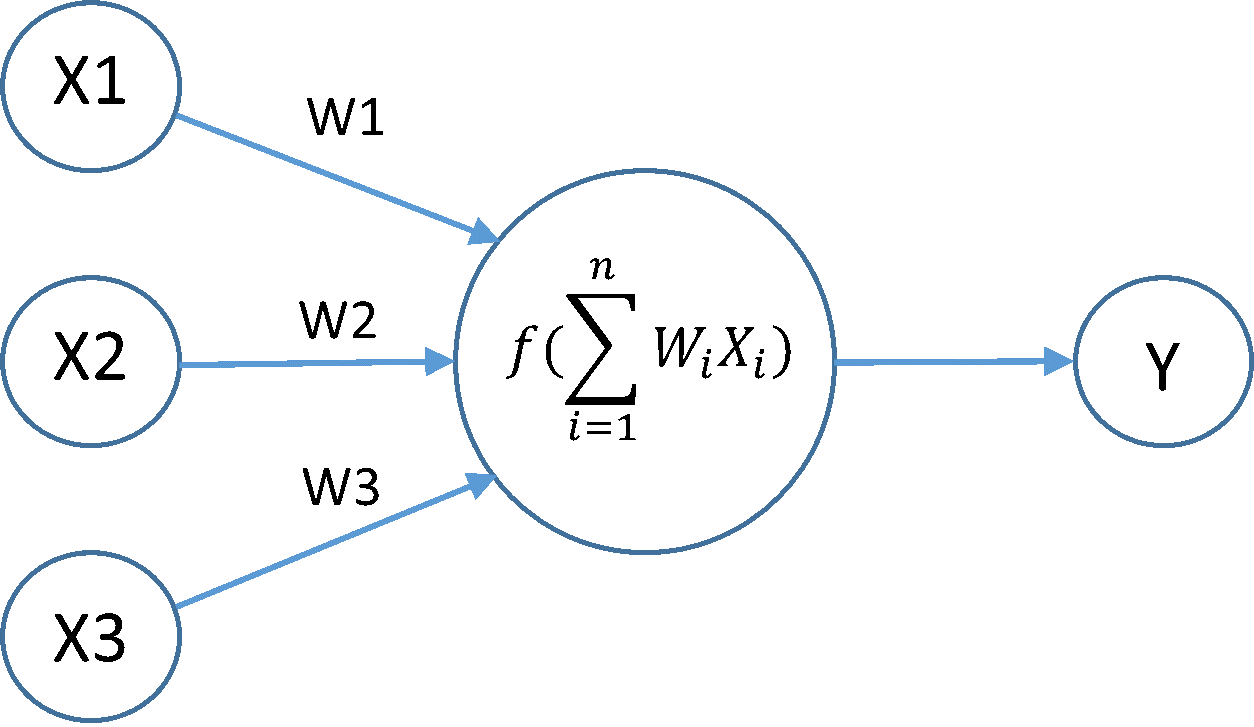
\includegraphics[width=3.5in]{photos/neuron}\\
  \caption{A simple Neuron with 3 inputs and 1 output \cite{neuron}}\label{neuron}
  \end{center}
\end{figure}

The range in which NN's (2020) can be applied nowadays is wide. Some disciplines have only been created due of the invention of neural networks, because they solve existing- and new problems very effective and efficiently. Many frequently held conferences around the globe contribute continuous evidence of the successes of neural networks. Among those various disciplines counts for example \textit{Pattern recognition} with Convolutional Neural Networks (CNN) \cite{cnn} or the famous \textit{CIFAR-10} dataset \cite{cifar}, where many amateurs \cite{tim} and experts attempt annually to further increase the accuracy of predicting the 10 different image classes. \\
The topic of this thesis \textit{textgeneration} is based from the Natural Language Processing discipline, \textit{NLP} for short. This field covers many other hot research topics, such as 

\begin{itemize}
\item Sentiment Analysis
\item Machine Translation
\item Speech Recognition
\item Text Generation (Neural Text Generation \textit{NTG})
\item Chatbots
\end{itemize}

Another term for textgeneration is denoted by \textit{Language Modelling}, because generators use the words and grammar as input for the model. In the past five years were mainly two approaches for modelling NLP, namely the \textbf{rule-based} system and the \textbf{template-based} system (Figure \ref{rules_based}) \cite{NTG2}. Today neural end-to-end systems are is \textit{State-of-the-Art} \cite{End_to_End}. These new systems offer more flexibility and scale with proportionately better results and less data is required, because the complexity and thus the neccessary computing power has increased. However, this fact leads to a complexity problem, because it becomes very difficult to understand the decisions of the neural network. The neural network is still to a large extent basically a \textit{black box}, although it gives surprisingly good results, especially in NLP. Nevertheless, neural network models for text processing are difficult to understand, so nowadays compromises between rule-based systems still have to be made and hybrid systems are most commonly used. 

\begin{figure}
  \begin{center}
  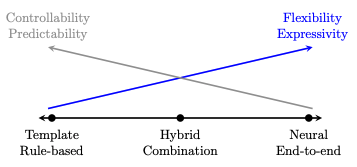
\includegraphics[width=3.5in]{photos/rule_based}\\
  \caption{Rule-Based vs. Neural-Text-Generations System \cite{NTG2}}\label{rules_based}
  \end{center}
\end{figure}

The neural text generation, also called \textit{NTG}, has many other interesting application fields, which overlap partly with NLP, including
\begin{itemize}
\item Speech recording and conversion to text
\item Conversation systems e.g. chatbots
\item Text summary
\end{itemize} 

In order to train language models, they must be taught the probability of occurring words in relation to the preceding words. There are several approaches to achieve this goal. Language models can be trained on the level of words, whole sentences or even whole paragraphs. The granularity in which the training takes place is called \textit{n-grams}, where \textit{n} represents the number of preceding words.

\section{Case study of a current NLP system}

To give an insight about a current use case, I will describe the basic architecture of the famous \textbf{Siri} from Apple. There are many very interesting use cases and I will further discuss the most important hot research topics of 2019-2020 in chapter \ref{ss:trends}, but Siri combines two of the most relevant NLP tasks, namely Speech Recognition and Text Generation. Siri was first released in 2011 for the iPhone 4s, but at this time, users were still required to press the \textit{Home Button} to give Siri a command. For Siri to fulfill the user commands, it needs to understand first the human language itself by recoginizing the words and generate the according text out of it. Secondly it needs to further process those words to a context and figure out what the user wants. 

\subsection{Hands-Free Access to Siri}
For the release of the iPhone 6 (iOS 8) in 2015, Apple upgraded Siri to a large extend. Without the need to interacting with the iPhone physically, it can now detect the primary-users voice \textit{"Hey Siri"} to wake up automatically. Even though it might not sound like an innovation, still a lot is going on behind the scences to create an flowless experience. The following figure \ref{flow} \cite{siri1} shows the process of detecting the wake-up sentence \textit{"Hey Siri"}.

\begin{figure}
  \begin{center}
  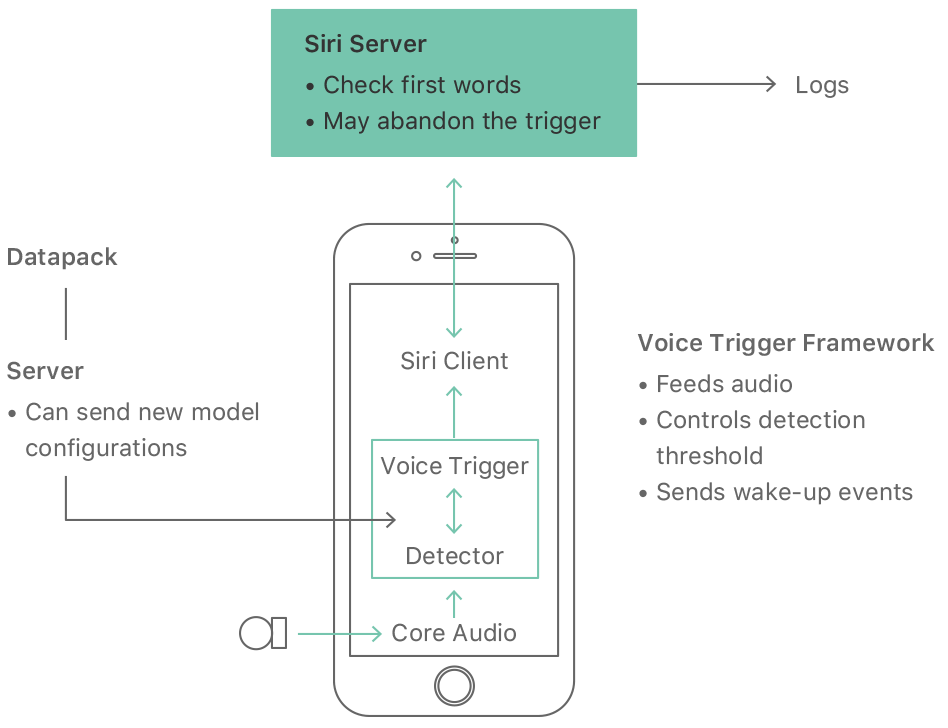
\includegraphics[width=4.5in]{photos/HeySiriFlow-1}\\
  \caption{The Hey Siri flow on iPhone (Apple 2017)\cite{siri1}}\label{flow}
  \end{center}
\end{figure}

Most of the high-tech technologies involved are stored on the cloud. The automatic speech recognition, the natural language interpretation and the various information devices are the major parts \cite{siri1}. \\
The core In figure \ref{flow} is basically the acoustic model. The iPhone microphone listens constantly and converts all sounds into a stream of waveform samples. Those samples are transformed into a sequence of frames, which describe approximately 0.01 seconds in time. Those frames are fed into the Deep Neural Network (DNN) acoustic model and produce a log probability to calculate the probabilty of the current sound being the \textit{"Hey Siri"} activation sentence. 
Adjustments to save the battery, limits of the processing capacities of the Centrul Processing Unit (CPU) and double security checks if the said senetence is really \textit{"Hey Siri"} are not revelant in this aspect.

\subsection{Personalized Hey Siri}
For the introduction of Apple's wake up feature \textit{"Hey Siri"} with the iPhone 6, Apple needs to use multiple machine learning and NLP technologies to function properly on all iPhones.
The first task is rather simpler compared to figuring out the context, but still highly researched. When it comes to programming, the language gets split up into basically three parts \cite{siri2}.

\begin{itemize}
\item \textit{Syntax}: Composition of the phrases
\item \textit{Semantics}: Meaning of the phrases
\item \textit{Pragmatics}: Composition and context of the phrases
\end{itemize}

Siri gets activated when it recognizes the words \textit{"Hey Siri"}. This is achieved through the use of Recurrent Neural Networks (RNN) \cite{siri2}, multi-style training and curriculum learning. The RNN will be further explained in chapter \ref{ss:nn}. Siri is able to avoid unintended activations which sound similar, but have a different meaning. This is especially challenging, because people all over the world have different accents and dialects, depending on their origins. 

When the phone is configurated, in the \textit{enrolment stage} the user is asked to repeat common phrases for a couple of times. This input is fed into a \textit{statistical model} for the user’s own voice. In the \textit{recognition stage}, the computer evaluates if the speech input fits to the primary-users-trained model accepts or rejects the request based on that decision.

	
\begin{figure}
  \begin{center}
  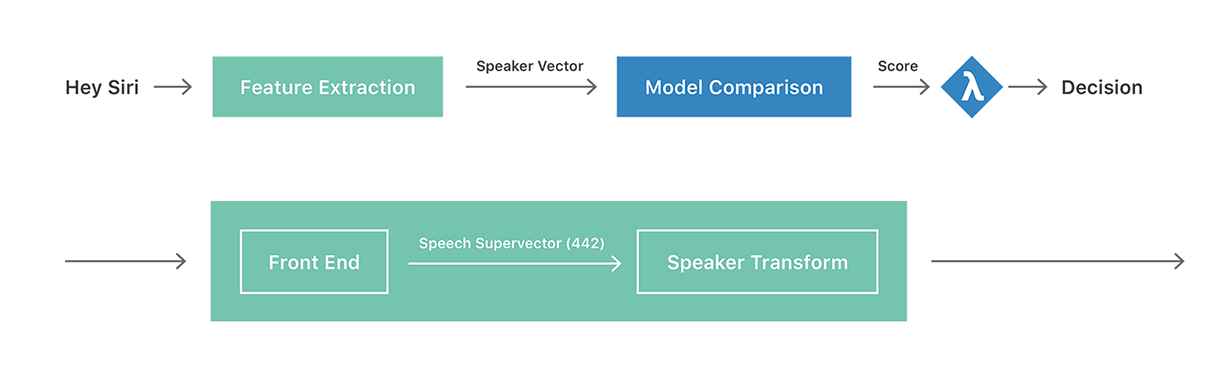
\includegraphics[width=4.5in]{photos/siri1}\\
  \caption{Block diagram of Personalized "Hey Siri" (Apple 2018)\cite{siri2}}\label{siri1}
  \end{center}
\end{figure}

Figure \ref{siri1} from Apple shows the very basic diagram for this process \cite{siri2}. The \textit{Feature Extraction} computes a fixed-length speaker vector for the input sentence \textit{"Hey Siri"}. This vector contains information about phonetics, background noise and the identity of the user. In the next step is the vector transformed in such a way, that the environmental background noise is being reduced to a minium with the help of the \textit{Fourier Transform}



